% !TEX root = MasterThesis.tex

\chapter{Modern Operating System Concepts}\label{ch:modern-os-concepts}
%
%https://groups.google.com/forum/#!topic/comp.os.minix/wlhw16QWltI%5B1-25%5D
 % 2: your job is being a professor and researcher: That's one hell of a
% good excuse for some of the brain-damages of minix. I can only hope (and
% assume) that Amoeba doesn't suck like minix does.
% >1. MICROKERNEL VS MONOLITHIC SYSTEM
% True, linux is monolithic, and I agree that microkernels are nicer. With
% a less argumentative subject, I'd probably have agreed with most of what
% you said. From a theoretical (and aesthetical) standpoint linux looses.
% If the GNU kernel had been ready last spring, I'd not have bothered to
% even start my project: the fact is that it wasn't and still isn't. Linux
% wins heavily on points of being available now.
%
This thesis' introduction already picked up the discussion about which operating system architecture is the superior one by refering to the \textit{Tanenbaum-Torvalds debate}\cite{linux-is-obsolete} in 1992.
Besides the discussion is quite interessting from todays view on different operating systems, the forecasts on their future and the actual development, are both, \textsc{Tanenbaum} and \textsc{Torvalds} underpinning their arguments with the origins of their implementations \textit{MINIX} and \textit{Linux} in different problems. 
And roughly spoken are exactly such different problems which needs to be solved with an operating system one reason for their diversity. 
Over the years, they had to fit in solving very different kinds of problems on very different kinds of hardware, which resulted in many different ways of working and architectures. 
As with the debate, it is rather difficult to impossible to find one architectural concept or implementation which is clearly superior to the other ones in every use-case. 
Nevertheless, it is a reasonable question why a majority of the operating system kernels which were developed from scratch in the last few years are based on a microkernel concept.
In 2009, the official statement of the Linux kernel developer \textsc{Richard Gooch} was still that monolithic kernels are superior for performance reasons\cite{why-linux-monolith}.
So the question remains what changed during the last ten years to promote this change, and especially for this work, how this affects on device driver development.
For this reason, this chapter is dedicted to the basic components and functionallities of operating system kernels and how they are implemented in the real world examples \textit{Linux} and \textit{Zircon}.


%%%%%%%%%%%%%%%%%%%%%%%%%%%%%%%%%%%%%%%%%%%%%%%%%%%%%%%%%%%%%%%%%%%%%%%%
% Links
%
% Some notes to Linux design decisions: \url{http://vger.kernel.org/lkml/#s15-3}
% Memory management in Linux -> Files from LFD 430
% 
%
%%%%%%%%%%%%%%%%%%%%%%%%%%%%%%%%%%%%%%%%%%%%%%%%%%%%%%%%%%%%%%%%%%%%%%%%


\section{Operating System Architectures}\label{sec:kernel-arch-concepts}

% TODO OS design goals see Betriebssysteme Glatz 
As already pointed out are architectural decisions for operating systems commonly influenced by the issues they are intended to solve.
By giving priority to some design objectives that are pertinent to the underlying issue, different concepts and architectures are the outcome.
According to \textsc{Glatz}\cite{glatz2015betriebssysteme} are some of them:
\begin{itemize}
    \item Providing a reliable, crash-proof environment.
    \item Providing a portable operating system.
    \item Providing a scalable operating system, e.g.\ in terms of processing cores.
    \item Providing an extensibile operating system, e.g.\ in terms of adding additional functionality to the kernel.
    \item Providing real-time capabilities.
    \item Providing an efficient design in terms of ressources and performance.
    \item Providing a secure environment for user applications.
    \item Providing a maintainable operating system, e.g.\ by the division of policy and mechanism. 
\end{itemize}\ \\
%
How these design principles fit into the known operating system architectures will be considered in the following sections.
But before, the terms \textit{kernel mode} and \textit{user mode} will be explained as they are fundamental for this work.

\subsubsection*{Dual-Mode Execution}
Modern general purpose \acp{cpu} provide a ring based, hardware enabled security model which had it's origin in the Intel x86 processor architecture\cite{tanenbaum-modern-operating-systems}.
It is usually made of four different security levels, the rings 0 to 3 which are illustrated in Figure~\ref{pic:x86rings}.
In this model, ring 3 is the least secure level, used for common user applications (even if started with \textit{root} privileges), while ring 2 is used for libraries shared between user applications and ring 1 is for system calls\cite{glatz2015betriebssysteme}.
System calls provide the transition to ring 0, the ring with the topmost security level, which is used for the operating system kernel.
As a crucial part of an operating system, they will be discussed in more detail later in this work.

Directly related to this model is the \textit{dual-mode} execution mode of modern \acp{cpu}.
It is a hardware enabled security concept to provide a distinction between the user applications in ring 3 and the actual operating system kernel in ring 0.
Just the kernel in ring 0, running in the \textit{kernel mode} (or \textit{privileged mode, supervisor mode or system mode}), has direct and privileged access to memory, hardware, timers or interrupts, e.g.\ for performing \ac{io} operatings or memory mapping\cite{lfd430}.
User applications in ring 0, running in the \textit{user mode}, are not allowed to them so directly, they have limited privileges and a limited instruction set.
As named above, they need to use a mechanism called \textit{system calls} to transfer the execution to the \textit{kernel mode} where the priviledged actions are performed.
Lastly, the execution is transfered back to the calling user process and with this, the mode changes back to \textit{user mode}.
Figure~\ref{pic:mode-switches} pictures the operating flow of a system call including the mode switches between \textit{user} and \textit{kernel mode}.

%
%
\begin{figure} [ht]
	\centering
	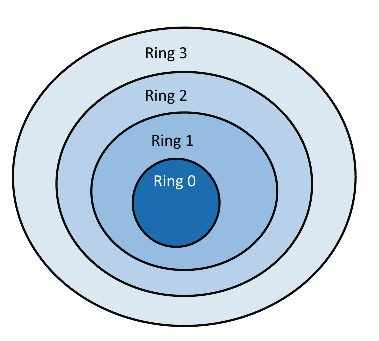
\includegraphics[scale=0.6]{x86Rings}
	\caption{The Rings of the x86's security concept\cite{glatz2015betriebssysteme}}\label{pic:x86rings}
    %TODO own picture!
\end{figure}
%
\begin{figure} [ht]
	\centering
	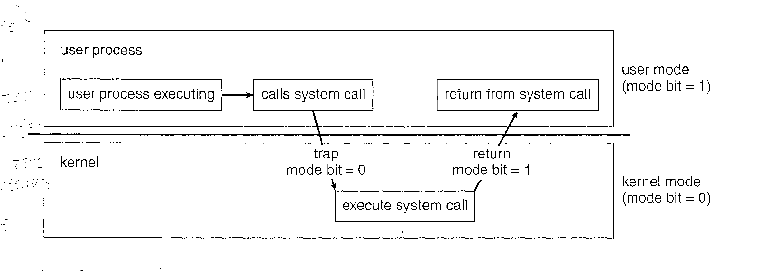
\includegraphics[scale=0.6]{mode-switch}
    \caption{A system calls sequence including the mode switches\cite{glatz2015betriebssysteme}}\label{pic:mode-switches}
    %TODO own picture!
\end{figure}

The \ac{cpu}'s operating mode is usually controlled by a specific bit in the \ac{psw}\cite{tanenbaum-modern-operating-systems}.
It influences the state of each \ac{cpu} core itself in a multi-processor system, but not the operating system kernel.
As a result, different \ac{cpu} cores may be in a different execution mode\cite{lfd430}.
With this seperation, any priviledged instruction is forbidden in \textit{user mode} and will not be executed.

Based on the dual mode execution on the \ac{cpu}, different architectural concepts for operating systems evolved.
They differ e.g.\ in the share of the operating system respectively the operating system's kernel actually running within the \ac{cpu}'s \textit{kernel mode}. 
Thus, they have an influence on the whole system, including device driver development but also on performance and security issues.
With this basic knowledge about the \ac{cpu}'s operating modes, the next section researches a selection of different operating system architectures.
Special attention should be paid to the most common ones, the \textit{monolithic} and the \textit{microkernel} architectures and their implementation in Linux and Zircon.

On the contrary, this work will not take a particular look on special purpose operating system architectures such as ones for loosely coupled multi-processor systems known from processing clusters.
Today, even the majority of general purpose computing systems are driven by more than one \ac{cpu} and most of common modern operating systems are designed to provide support for the defacto standard for tightly coupled systems, \ac{smp}.


\subsection{Monolithic Architectures}

% \cite{lfd430}, Appendix A

\subsection{Microkernel Architectures}
% TODO Why are microkernel interesting and nearly each new developed one is a microkernel?
\subsection{Layered Architectures}
% \subsection{Distributed Architectures}
\subsection{Hybrid Architectures}
\subsection{The Linux Kernel's Monolithic Architecture}
% TODO mischformen
% TODO actual Linux architecture, mixed form of monolith, module concept
\subsection{The Zircon Kernel's Microkernel Architecture}
% TODO actual Zircon architecture, overview


\section{System Calls}\label{sec:system-calls}
% TODO normally are system calls a part of the section processes and threads,
% but for the reason zircon is very special there (not fully POSIX compatible),
% it shall be handled with more respect in this work
% (If it will work)? -> it should -> Achilles Betriebssysteme
% Tanenbaum 1.6
% Operating system concepts 8.edition 2.3
% Betriebsysteme Grundlagen und Konzepte 1.3.1
\subsection{POSIX}
\subsection{System Calls in Linux}
\subsection{System Calls in Zircon}
% FIDL, core libs,.. 


\section{Processes and Threads} %TODO label
\subsection{Processes}
\subsection{Threads}
\subsection{Inter Process Communication}
\subsection{Scheduling}
\subsection{Processes and Threads in Linux}
\subsection{Processes and Threads in Zircon}


\section{Memory Management} %TODO label
%    Linux Concept -> LFD430 pic
%TODO find sections
%TODO how is it done in Linux and Zircon
\subsection{Address Spaces}
\subsection{Virtual Memory}
\subsection{Page Replacement/Paging}
\subsection{Memory Management in Linux}
\subsection{Memory Management in Zircon}


\section{I/O} %TODO label
%TODO review sections, how is it done in Linux/Zircon
\subsection{I/O Hardware}
\subsection{Memory Mapped IO}
\subsection{Direct Memory Access}
\subsection{Interrupts}
\subsection{Power Management}

   
\section{Security Concepts} %TODO label
\subsection{Access Control} %Domains, Capabilities
%DAC, MAC, ..
\subsection{Security Concepts in Linux}
\subsection{Security Concepts in Zircon}


\section{Driver Models} %TODO label
